
\hypertarget{basic_faq}{}
\section{FAQ}
\index{FAQ}

This section provides information on \textbf{F}requently \textbf{A}sked
\textbf{Q}uestions (FAQ).


\subsection{What is Tinn-R?}
\index{FAQ!What is Tinn-R?}
\index{What is Tinn-R?}

\begin{itemize}
  \item \htmladdnormallink{Tinn}{http://tinn.solarvoid.com} is a small
    ASCII file editor primarily intended as a better replacement for
    the default Notepad running under the Windows OS. The name is the
    recursive acronym: \underline{T}inn \underline{i}s \underline{n}ot
    \underline{N}otepad.
  \item \htmladdnormallink{Tinn-R}{http://nbcgib.uesc.br/lec/software/editores/tinn-r/en}
    is an extension of the original Tinn editor, providing additional
    functionality to control
    \htmladdnormallink{R}{http://cran.r-project.org}
    running as Rgui (in SDI mode), Rterm,
    \htmladdnormallink{SciViews R}{http://www.sciviews.org/SciViews-R}
    console and
    \htmladdnormallink{JGR}{http://stats.math.uni-augsburg.de/JGR/}.
    And a whole lot of additional resources.
  \item Tinn-R can also be thought of as feature-rich replacement of the
    basic script editor provided with Rgui. It provides syntax-highlighting,
    code submission as a whole or line-by-line, in addition to many other
    useful tools to ease the writing and debugging of \RR{} code.
  \item Both Tinn and Tinn-R are distributed under the
    \htmladdnormallink{GPL 2}{http://www.gnu.org/copyleft/gpl.html}
    license or above.
\end{itemize}


\subsection{Feedback, suggestions and bug report}
\index{FAQ!feedback}
\index{feedback}
\index{FAQ!suggestions}
\index{suggestions}
\index{FAQ!bug report}
\index{bug report}

Please send your feedback to
\htmladdnormallink{Jos� Cl�udio Faria}{mailto:joseclaudio.faria@gmail.com}.
If you submit a bug report, please provide as much detail as possible. This
includes indicating the Tinn-R version, your operating system (Windows XP,
Windows 7, etc), and language (English, French, Portuguese). If the bug
is related to an interface with \RR{}, please also indicate which version of
\RR{} you are using, as well as whether you are running Rterm or Rgui. Ideally,
please also add the content of the \textit{Tools/Results/Ini log}
interface since this will help us address the issue more promptly.


\subsection{Tinn-R installation}
\index{FAQ!Tinn-R installation}
\index{Tinn-R installation}

\textit{\htmladdnormallink{See details ...}{\#basic\_configuration}}


\subsubsection{Where can I get the latest version of Tinn-R?}
\index{FAQ!latest version}
\index{latest version}

\begin{itemize}
  \item The latest version of Tinn-R can be downloaded from
    \htmladdnormallink{Web page}{http://nbcgib.uesc.br/lec/software/editores/tinn-r/en} or
    \htmladdnormallink{SourceForge}{https://sourceforge.net/projects/tinn-r/}.
\end{itemize}


\newpage
\subsubsection{How do I install Tinn-R?}
\index{FAQ!install}
\index{install}

\begin{itemize}
  \item Tinn-R uses a classical method of installation and runs on all
    versions of the Windows OS. You need administrative rights to install,
    although you can install it as a regular user provided you have
    write permission on the directory where you will perform the installation.
    If you have problems, please contact your computer or network
    administrator.
  \item Note that if you install Tinn-R you will likely want to use
    it along with \RR{}, and so \RR{} must be installed separately.
    \RR{} can be obtained from
    \htmladdnormallink{here}{http://cran.r-project.org}.
\end{itemize}


\hypertarget{faq_trpaths}{}
\subsubsection\textbf{.trPaths? (a very recorrent FAQ)}
\index{FAQ!.trPaths?}
\index{.trPaths?}

If your version is the same or above 3.0.1.0, Tinn-R does not require any special configuration.
That is, the program is ready to be used. One important thing to be done before using it:
set a \RR{} mirror as close as possible to where you work. For that, first click on \texttt{CTRL + F8}.
This opens the \texttt{Tools} window, then click on \texttt{R/Mirrors}.
Select the \RR{} mirror and push the button that shows an hourglass in the taskbar.
The chosen repository will be the new default for all actions dependent repository
(install packages, upgrade packages, etc).

If you have any version of Tinn-R ($<$= 2.2.0.2) installed,
you need to define your .trPaths correctly in the file \texttt{R/etc/Rprofile.site}.
With the "new" versions of Windows (Vista, 7 e 8) write permissions are more annoying to deal with,
and you have to manually give yourself permission to write to the file/directory,
before you can change and save the files. So, to fix it, you have to enable write
access to the \texttt{Rprofile.site} file and then configure \RR{} to run.

\begin{itemize}
  \item Locate your \RR{} install. The default is \texttt{C:$\backslash$Program Files$\backslash$R$\backslash$R-X.X$\backslash$}.
  \item The file you need write access to is \texttt{Rprofile.site}, located in the folder \texttt{etc}.
    A good option is to give write access to all of \texttt{C:$\backslash$Program Files$\backslash$R$\backslash$R-X.X$\backslash$}.
  \item Select the directory you want to give yourself permission to write in, right click, properties,
    security, and then it depends on your version of Windows. Once you've enabled writing and saved, you'll need to go back to Tinn-R.
    In the main menu choice: \texttt{R/Configure/Permanent(Rprofile.site)}.
  \item It should autoload and fix your \texttt{Rprofile.site} file.
  \item The one additional change you would make is to either comment out or change your default repository.
  \item Usefull links about:
    \begin{enumerate}
      \item Hidden (files and folders)
        \begin{itemize}
          \item \htmladdnormallink{Microsoft}{http://windows.microsoft.com/en-US/windows7/Show-hidden-files}
          \item \htmladdnormallink{Carbonite}{http://carbonite.custhelp.com/app/answers/detail/a\_id/1379/\~{}/\%5Bwindows\%5D-viewing-hidden-files-and-folders}
          \item \htmladdnormallink{About.com}{http://pcsupport.about.com/od/windows7/ht/show-hidden-files-windows-7.htm}
          \item \htmladdnormallink{Computer Hope}{http://www.computerhope.com/issues/ch000516.htm}
        \end{itemize}
      \item Permission (files and folders)
        \begin{itemize}
          \item \htmladdnormallink{Microsoft}{http://windows.microsoft.com/en-US/windows-vista/Troubleshoot-access-denied-when-opening-files-or-folders}
          \item \htmladdnormallink{Seven Forums}{http://www.sevenforums.com/tutorials/122666-permissions-allow-deny-users-groups.html}
          \item \htmladdnormallink{Addictive Tips}{http://www.addictivetips.com/windows-tips/windows-7-access-denied-permission-ownership/}
        \end{itemize}
    \end{enumerate}
\end{itemize}


\subsubsection{Can I get the source code?}
\index{FAQ!source code}
\index{source code}

\begin{itemize}
  \item Yes. You can get and modify the source code of Tinn-R as well
    as redistribute your changes as long as you respect the terms of
    the GPL license. The source code is available from
    \htmladdnormallink{SourceForge}{https://sourceforge.net/projects/tinn-r/}.
\end{itemize}


\subsubsection{How can I add a shortcut to Tinn-R in the start menu or in the desktop?}

\begin{itemize}
  \item This is automatically done by the installer.
    If you want to do it manually later on, here are the steps:
    \begin{enumerate}
      \item Under object explorer, right-click the file \texttt{Tinn-R.exe}
        and select \texttt{Create shortcut};
      \item Drag \& drop this shortcut to the desktop or wherever you
        might want to place it.
    \end{enumerate}
\end{itemize}


\hypertarget{faq_preferences}{}
\subsubsection{Can I save or reuse my preferences on another computer?}
\index{FAQ!save my preferences}
\index{save my preferences}
\index{FAQ!reuse my preferences}
\index{reuse my preferences}

\begin{itemize}
  \item You have a save/restore configuration tool under
    \texttt{Tools/Backup or Restore system configuration} or \texttt{Database}.
    Just backup your config file on one computer, copy it to the computer
    where you intend to use the same preferences, then restore them there.
  \item The restore function assumes that you are using same OS and user name.
  \item Otherwise:
    \begin{enumerate}
      \item Unzip the file Tinn-R\_X.X.X.X\_preferences\_bkp in a place of
        your choice;
      \item Copy the folder Tinn-R;
      \item Paste it inside the directory with the Tinn-R folder;
      \item To find where that folder is located, from the main menu
        just select \texttt{Help/Ini files (path information)}.
    \end{enumerate}
\end{itemize}


\subsubsection{How can I open a file in Tinn-R by double-clicking it under Windows Explorer?}

\begin{itemize}
  \item You need to register Tinn-R as the default program to open
    files with a given extension. You can either check this
    option during installation or follow the steps below:
    \begin{enumerate}
      \item In order to open *.R files (\RR{} scripts) with Tinn-R, locate
        one such file in your disk;
      \item Right-click this file and select \texttt{Open
          with/Choose program...} in the context menu;
      \item Click \texttt{Browse} in the \texttt{Open with} dialog
        box and then select \texttt{Tinn-R.exe};
      \item Make sure the option \texttt{Always use the selected
          program to open this kind of file} is selected;
      \item Click \texttt{OK}.
    \end{enumerate}
  \item Now, when you double-click on a *.R file in the Windows
    explorer, it will be opened in Tinn-R.
\end{itemize}


\newpage
\subsubsection{How to define the starting Rgui from within Tinn-R?}
\index{FAQ!starting GUI}
\index{starting GUI}

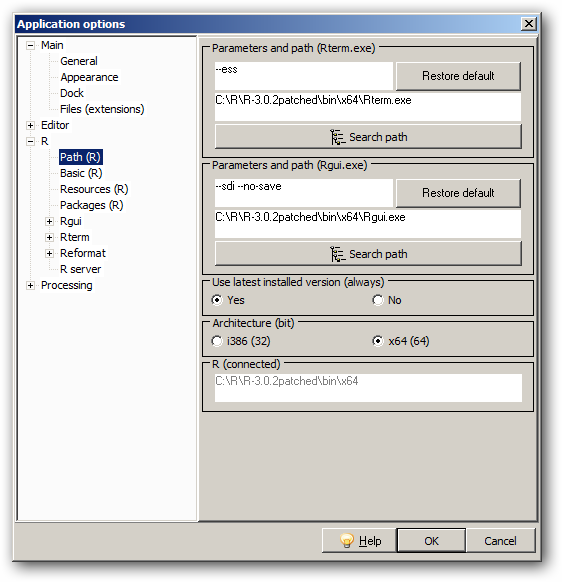
\includegraphics[scale=.50]{./res/app_r_path.png}

\begin{itemize}
  \item You can start your preferred Rgui directly from Tinn-R. To do that,
    go to \texttt{Options/Application/R/Path}.
  \item At the bottom of the dialog box, you can determine the path of
    the Rgui executable to start from within Tinn-R. Select
    \texttt{Rgui.exe} from, for instance,
    \texttt{C:$\backslash$Program Files$\backslash$R$\backslash$R-X.X.X$\backslash$bin$\backslash$Rgui.exe}).

    \begin{footnotesize}
      \begin{verbatim}
        Note: to use R from within Tinn-R, you must first install it from
        http://cran.r-project.org
      \end{verbatim}
    \end{footnotesize}

  \item With Rgui, you must choose SDI mode at Edit/GUI preferences.
\end{itemize}


\subsubsection{Can I define Tinn-R as the default editor for R objects?}
\index{FAQ!default editor}
\index{default editor}

\begin{itemize}
  \item No, currently, it does not have that capability. In order to do that,
    just use the internal script editor of Rgui to edit() or fix() \RR{} objects.
\end{itemize}


\subsubsection{Can I use Emacs or WinEdt style for syntax highlighting color?}
\index{FAQ!Emacs}
\index{Emacs}
\index{FAQ!WinEdt}
\index{WinEdt}

\begin{itemize}
  \item Just set your preferred color scheme in \texttt{Options/Colors (preference)}.
    To change color scheme on other computers, just use the
    \texttt{Options/Backup/Restore system options} configuration functions
    (\textit{\htmladdnormallink{See details ...}{\#faq\_preferences}}).
\end{itemize}


\subsubsection{What does "Triggers" mean in Options/Application/R/General/Basic?}
\index{FAQ!triggers}
\index{triggers}

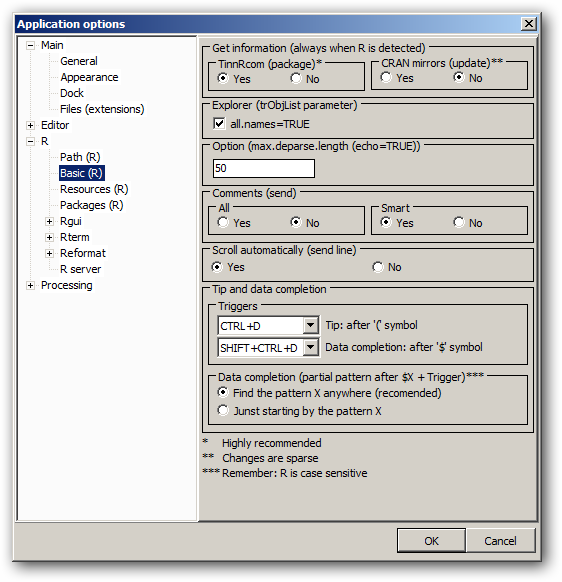
\includegraphics[scale=.50]{./res/app_r_basic.png}

\begin{itemize}
  \item Tips are tooltips displaying the syntax of the currently used
    \RR{} function.
  \item By default, if you enter the name of a function followed by an open
    bracket such as \texttt{sd(} in a \RR{} code document, then Tinn-R recognizes
    that you call the \texttt{sd} \RR{} function and reminds you of its syntax
    by showing the following tip: \texttt{x, na.rm=FALSE}, that is, \texttt{sd}
    accepts two arguments: \texttt{x}, and \texttt{na.rm} with the latter
    having \texttt{FALSE} as the default value.
  \item Tinn-R uses a database with the syntax of most common functions in \RR{}.
    However, neither functions in additional packages nor your custom
    functions are cached in this database.  Adding them all manually is
    tedious.
  \item Tinn-R therefore offers a second mechanism: direct requests to \RR{}. This
    is accomplished through DDE and/or TCP/IP protocols, using functions
    automatically loaded when you start the TinnR package you downloaded
    from CRAN.
    (\textit{\htmladdnormallink{See details ...}{\#basic\_configuration}}).
  \item When a tip is showed (Editor, IO or Log interface) it is possible
    to add all arguments by typing the shortcut \texttt{CTRL + *}.
\end{itemize}

On some computers, the delay for synchronization might need to be adjusted.
If Tinn-R seems to freeze while querying \RR{} for tips and you get no results,
increase the value a bit by setting
\texttt{Options/Application/Main/General/Computational synchronization (delay)}.


\subsubsection{Can I start R and Tinn-R all at once?}

\begin{itemize}
  \item There are many ways to accomplish this, but here is one: first,
    configure \RR{} so that it undersands that you want to use Tinn-R
    as your IDE (Integrated Development Environment). In order to do
    that, start a new \RR{} session and add the following command:

    \begin{footnotesize}
      \begin{verbatim}
        > options(IDE = "C:/Tinn-R/bin/Tinn-R.exe")
      \end{verbatim}
    \end{footnotesize}

    Replace the path by the present location of Tinn-R.exe on your computer
    if different from the location above. Then you will indicate that you
    want to start the DDE server automatically by setting (valid only for
    versions prior to 3.0.1.0, because this communication protocol
    was deleted from the project, the only one remaining is TCP/IP):

    \begin{footnotesize}
      \begin{verbatim}
        > options(use.DDE = TRUE)
      \end{verbatim}
    \end{footnotesize}


    At this point, Tinn-R will be automatically started when you load svIDE,
    at the same time as the \RR{} call-tip server is installed (valid only for
    versions prior to 3.0.1.0):

    \begin{footnotesize}
      \begin{verbatim}
        > library(TinnR)
      \end{verbatim}
    \end{footnotesize}

    If those steps work well in manual mode, but you now want them to run whenever
    you start \RR{}, edit the \texttt{Rprofile.site} file (located in the
    $\backslash$etc$\backslash$ subdirectory of \RR{}.  File location varies, but
    it should be under something like
    C:$\backslash$Program Files$\backslash$R$\backslash$R-X.X.X$\backslash$etc$\backslash$Rprofile.site).
    Add the above-mentioned three lines of code at the end of the Rprofile file (valid only for
    versions prior to 3.0.1.0).

    \begin{footnotesize}
      \begin{verbatim}
        options(IDE = "C:/Tinn-R/bin/Tinn-R.exe")
        options(use.DDE = TRUE)
        library(TinnR)
      \end{verbatim}
    \end{footnotesize}

    A copy of \texttt{Rprofile.site} file created by Jos� Cl�udio Faria can be obtained from
    \htmladdnormallink{SourceForge}{http://sourceforge.net/p/tinn-r/news/2013/01/rprofilesite-example/},
    which you can adapt according to your needs. To make sure that everything works well and
    smoothly, close both \RR{} and Tinn-R and restart \RR{}. Tinn-R should start concomitantly.
    Now, create a very simple function in \RR{} such as:
    \index{installation!sourceforge}

    \begin{footnotesize}
      \begin{verbatim}
        > cube <- function(x) x^3
      \end{verbatim}
    \end{footnotesize}

    Switch to Tinn-R and type: \texttt{cube(}. You should get a call-tip displaying
    \texttt{x} if the \RR{} call-tip server was correctly installed.

\end{itemize}


\subsection{Hotkeys (operational system)}
\index{FAQ!hotkeys}
\index{hotkeys}

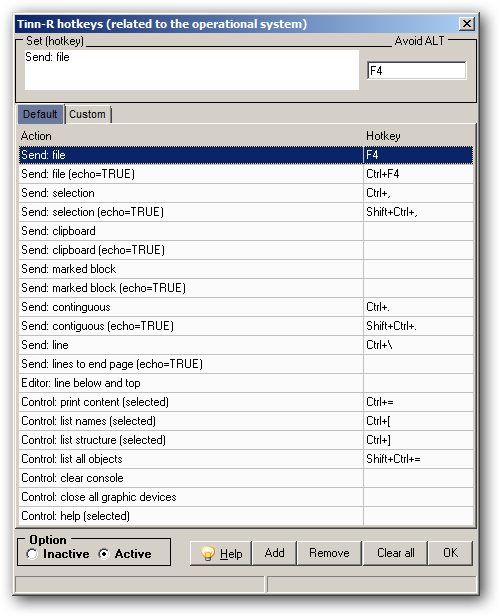
\includegraphics[scale=.50]{./res/hotkeys_default.png}
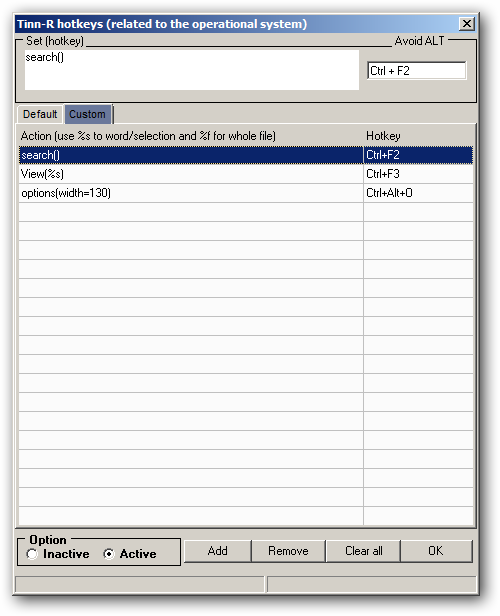
\includegraphics[scale=.50]{./res/hotkeys_custom.png}

\subsubsection{What is the difference between hotkeys (operational system) and shortcuts in Tinn-R?}

\begin{itemize}
  \item The hotkeys are related to the operational system. In other
    words, they work without the focus on Tinn-R, whereas the
    shortcuts will only work with the focus on the Tinn-R interface.
\end{itemize}


\subsubsection{How do I define hotkeys for R tools in Tinn-R?}
\index{FAQ!defining hotkeys}
\index{defining hotkeys}

\begin{itemize}
  \item Go to \texttt{R/Hotkeys of R}. Once there, define your favorite
    hotkeys for the various \RR{} tools and make sure to activate them
    (Option -$>$ Active).
\end{itemize}


\newpage
\subsubsection{Is there a shortcut for cycling through opened files?}
\index{FAQ!shortcut for cycling}
\index{shortcut for cycling}

\begin{itemize}
  \item Yes, you can use \texttt{CTRL + TAB} to go to next file, and
    \texttt{CTRL + SHIFT + TAB} to go to previous ones when several
    files are loaded simultaneously in Tinn-R.
\end{itemize}


\subsubsection{Is there a shortcut for $<$- and -$>$ for the S/R languages?}

\begin{itemize}
  \item The (non user configurable) shortcut for \texttt{-$>$} is
    \texttt{CTRL + ADD} key (numeric keypad). Similarly,
    \texttt{CTRL + SUBTRACT} (numeric keypad) is a shortcut for
    \texttt{$<$-}. \texttt{-$>$} and \texttt{$<$-}, all being
    assignment symbols in the S/R languages.
\end{itemize}


\subsection{Miscellaneous}

\subsubsection{I am editing a table. Can I select text in column mode?}
\index{FAQ!column mode}
\index{column mode}

\begin{itemize}
  \item Yes you can, but you must first make sure that this option is selected.
    Go to \texttt{Options/Application/Editor/Advanced options} tab and check (x)
    \texttt{Alt sets column modes}. Once this is done, by pressing
    \texttt{Alt} key while selecting your text with the mouse in Tinn-R,
    the  selection will be done in column mode.
  \item Another option is to change the selection mode to column in a permanent
    way. This is done through the menu \texttt{Options/Selection mode} or by
    clicking on the selection mode place at the status bar. The available
    options are: \texttt{smNormal}, \texttt{smLine} and \texttt{smColumn}.
\end{itemize}


\subsubsection{Can I define bookmarks to facilitate the navigation through my documents?}
\index{FAQ!bookmarks}
\index{bookmarks}

\begin{itemize}
  \item Yes, you can define up to 10 bookmarks in each of your opened documents.
    To define the bookmark, use \texttt{CTRL + SHIFT + [0-9]} (a key from 0 to 9).
    Then, to go to the corresponding bookmark just use \texttt{CTRL + [0-9]}.
    A visual indicator appears in the right margin at the location of your
    bookmarks to remind you where they are.
\end{itemize}


\newpage
\subsubsection{What is the left gutter used for?}
\index{FAQ!gutter}
\index{gutter}

\begin{itemize}
  \item In Tinn-R, bookmarks are visually displayed in the left gutter
    (use \texttt{CTRL + SHIFT + [0-9]} to set bookmarks and then use
    \texttt{CTRL + [0-9]} to navigate to them). It also displays the
    respective line numbers. You must set gutter \texttt{Visible} in
    \texttt{Options/Application/Editor/Display tab} (and also
    \texttt{Show line numbers}) to activate this feature.
\end{itemize}


\subsubsection{Can I run my code step-by-step?}
\index{FAQ!step-by-step}
\index{step-by-step}

\begin{itemize}
  \item Yes, but for more convenient use of this function, you must
    place Tinn-R and \RR{} side by side on your screen and click on the
    'Send line' icon with the mouse (seventh button from the left
    on the \RR{} toolbar).
  \item If you use a shortcut, you can just submit one line since the
    \RR{} console gets the focus when code is sent to \RR{}. Alternatively,
    you can set Tinn-R as a \texttt{topmost} window on top of \RR{}
    using \texttt{Options/On top}. The downside is that Tinn-R
    will permanently hide the \RR{} console and there is a chance
    that you won't see a part of the output generated in \RR{} during
    your step-by-step code execution.
\end{itemize}


\subsubsection{Is there a graphical debugger for my R functions?}
\index{FAQ!graphical debugger}
\index{graphical debugger}

\begin{itemize}
  \item Not yet, but you can download the excellent \texttt{debug}
    package from CRAN and use the \texttt{mtrace} function available
    from there.
\end{itemize}


\subsubsection{What is the Tools panel?}
\index{FAQ!tools panel}
\index{tools panel}

\begin{itemize}
  \item It is a panel you can open at either the left or the right
    side of your text. It helps you to manage large projects with
    multiple documents. The \texttt{Computer} tab allows you to
    explore your computer disks and open one or several files
    without using \texttt{File/Open}, or switching to the Windows
    file explorer. The \texttt{Project} tab is a convenient manager
    for all files collected in a given project.
\end{itemize}


\subsubsection{Can I copy and paste syntax highlighted R code in Word/Web/LaTeX?}
\index{FAQ!copy and paste}
\index{copy and paste}

\begin{itemize}
  \item Syntax highlighted code enhances the code's visibility. It is
    convenient in the code editor, but could also be useful for
    pieces of code presented elsewhere such as in a report, a Web
    page, or a LaTeX document. Tinn-R allows you to copy the code while
    keeping syntax highlighting color through \texttt{Edit/Copy
      formatted}. Three options are available: RTF, HTML and TeX.
\end{itemize}


\subsubsection{How can I fix incorrect icon displays on Windows after I have installed a new version of Tinn-R?}
\index{FAQ!icon on Windows}
\index{icon on Windows}

\begin{itemize}
  \item If you get an incorrect icon displayed on Windows after
    installing a new version of Tinn-R, just proceed as follows:
    \begin{itemize}
      \item In order to accelerate the display of program or file
        icons, Windows stores images in the ICON CACHE (ShellIconCache),
        a hidden icon cache file in your Windows directory.
      \item Sometimes the icon of the object changes, but Windows still
        shows the old icon instead of the new one. To solve this
        problem, use the shareware program called
        \htmladdnormallink{IconChanger}{http://www.shelllabs.com/}.
      \item If you have just installed Tinn-R with a new icon but Windows
        has not changed the image yet, use IconChanger and select REBUILD
        ICON CACHE.  If that still doesn't work, then select REMOVE ICON CACHE.
      \item If you have selected REBUILD the icon cache will start rebuilding
        from scratch. If you have selected REMOVE, you will see a warning
        message. Select YES and then restart your computer.
    \end{itemize}
\end{itemize}


\subsubsection{Basic instructions about focus control:}
\index{FAQ!focus control}
\index{focus control}


\includegraphics[scale=0.50]{./res/focus.png}
\begin{itemize}
  \item Tinn-R has a button within the \textit{Options toolbar}
    with the hint (\textit{Options: return focus to editor
      after send/control Rgui}) that enables the user to
    configure out the focus control. When this option is
    \texttt{checked} Tinn-R will display the following behavior:
    \begin{itemize}
      \item If the editor has the focus, it will \texttt{go back}
        to the editor after any \textit{send to} or \textit{R control}
        action, otherwise it will remain on Rgui. This is also
        true when working with a dual-monitor display.
    \end{itemize}
  \item If the Rterm has the focus, it will be \texttt{maintained}
    in this interface (\textit{IO}), \texttt{disregarding} the
    \textit{Options: return focus to editor after send/control
      Rgui}.
\end{itemize}


\newpage
\subsubsection{Why Tinn-R doesn't remember my syntax color preferences?}\\
\index{FAQ!color preferences}
\index{color preferences}

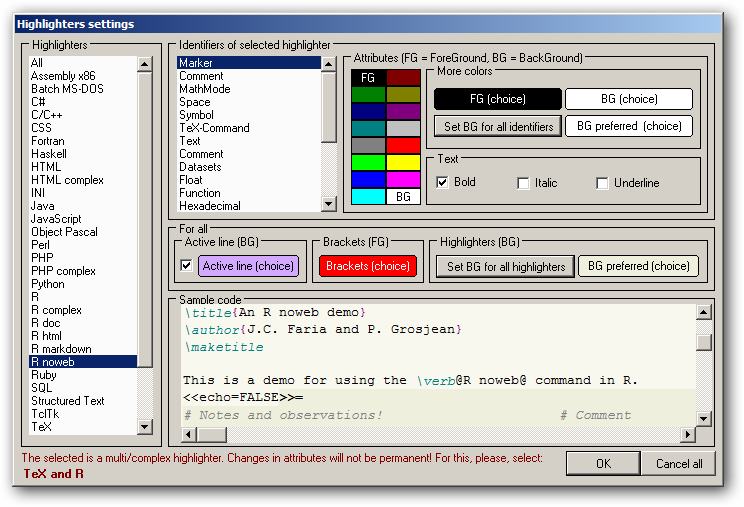
\includegraphics[scale=.50]{./res/highlighter_settings.png}

Tinn-R has seven multi-highlighters: \textit{HTML complex}, \textit{PHP complex},
\textit{R complex}, \textit{R doc},  \textit{R html}, \textit{R markdown} and \textit{R noweb},
with each one behaving as follows:

\begin{footnotesize}
  \begin{verbatim}
    1. HTML complex = HTML & JavaScript
    2. PHP complex  = HTML & JavaScript & PHP
    3. R complex    = R & URI ('<<<' begin URI; '>>>' end URI)
    4. R doc        = TeX & R ('>>=' begin R; '@' end R)
    5. R html       = HTML & R ('<!--begin.rcode' begin R; 'end.rcode-->' end R)
    5. R markdown   = URI & R ('```{' begin R; '```' end R)
    6. R noweb      = TeX & R ('>>=' begin R; '@' end R)

    URI       : Uniform Resource Identifiers.

    R complex : The main syntax is R, '<<<' and '>>>' are the tags enabling
                the user to insert a block of URI syntax.

    R doc     : The main syntax is TeX, '>>=' and '@' are the tags enabling
                the user to insert a block of R syntax.

    R html    : The main syntax is HTML, '<!--begin.rcode' and 'end.rcode-->' are the tags enabling
                the user to insert a block of R syntax.

    R markdown: The main syntax is URI, '```{' and '```' are the tags enabling
                the user to insert a block of R syntax.

    R noweb   : The main syntax is TeX, '>>=' and '@' are the tags enabling
                the user to insert a block of R syntax.

  \end{verbatim}
\end{footnotesize}

These highlighters do not establish priorities when you set the syntax color
preferences. Thus, if you change the color preferences for any of these
multi-highlighters these settings will be valid only
in the current Tinn-R session and will not be saved when Tinn-R is closed.
If you want to make these changes permanent, just set the  preferences
from all simple highlighters.


\subsubsection{How do I set a block as marked?}
\index{FAQ!marked blocks}
\index{marked blocks}

\begin{itemize}
  \item \textbf{If the file has no marks}: the option will not be
    available (grayed out);
  \item \textbf{If the file has one or more marks and the cursor
      is either above the first mark or below  the last mark}:
    all text (above or below this mark) will be submitted in
    relation to the cursor position (above or below) the mark;
  \item \textbf{If the cursor is between any two adjacent marks}:
    all text between those two marks will be submitted.
\end{itemize}


\subsubsection{How can I find errors in my script using Rterm interface?}
\index{FAQ!find errors in my script}
\index{find errors in my script}

\begin{itemize}
  \item The \texttt{Application options/R/Rterm} is split in two tabs: \texttt{Error} and \texttt{Options}.
    The tab Error has an option: \texttt{Trying to find code errors (at the editor)*}.
    It enables the user to set Tinn-R in order to find code errors at the editor when sending instructions to Rterm.
  \item It may happen that the error will not be found at the right place.
    For example, the error might be the same word
    appearing in a comment which comes before the actual code.
    In that case the user should use the shortcut \texttt{F3 (Find again)}.
    The word will appear selected, than just press \textit{OK} until finding the right error.
    The first search done internally by Tinn-R has \textit{Case sensitive} and \textit{Whole word only} as default,
    but, this is not passed to the search interface, therefore the user should just select them if convenient.
    If the error has numbers among letters \textit{Whole word only} is not a good option.
\end{itemize}


\subsubsection{The comunication between Tinn-R and Rgui seems to freeze!}
\index{FAQ!comunication}
\index{comunication}
\index{FAQ!Tinn-R and Rgui}
\index{Tinn-R and Rgui}
\index{FAQ!freeze}
\index{freeze}

\begin{itemize}
  \item \textbf{First, it is not necessary to reinstall the Tinn-R nor R}!
  \item In some Windows flavors the communication between \texttt{Rgui} and \texttt{Tinn-R} sporadically seems to freeze.
    The cause of this bug is still unknown to us and seems to be related to the new features of some Windows flavors.
    However, the solution is very simple: rest your mouse (without pressing for a few seconds) on the
    icon of the Tinn-R on the taskbar of windows\ldots: the communication should be restored automatically.
\end{itemize}
